\chapter{Layout recognition for tabular data}

Layout recognition is the process of extracting individual image elements and determining their logical relations. When applied to tabular data, its goal is to determine the presence and content of image tables. 

The extraction of table structures from a page poses various difficulties. Complications mostly arise when the input document does not correspond to the typical one-column, graphics-free layout. This may cause the spaces between individual page columns to be interpreted as table column spaces, which may lead to a complete rejection of any tables present in page columns. Additionally, complex layouts often cause difficulties when determining the reading order of the document. Therefore, in most cases, a \emph{layout analysis} first needs to performed.

\section{Layout analysis}

Layout analysis is the process of identifying and categorizing image document elements, such as figures, tables, forms, math symbols, headers, footers or simple paragraph text (\emph{geometric layout analysis}) and semantically labeling them according to their logical roles (\emph{logical layout analysis}).

In the previous chapter, we already covered the basics of geometric layout analysis, which is the same process as page segmentation~(\cref{pageSegmentation}). The output of this process is a data structure containing information about the detected elements. A logical layout analysis is then applied on this output.

Logical layout analysis is used to determine the reading order of the image document. It adopts the idea of \emph{labels}, which provide an information about the semantic order and type of individual document elements. For example, a label might be just a number indicating the reading order (as presented in~\cref{fig:readingOrderExample}), or it could contain more complex information, such as ``table header'', ``page footer'', ``image caption'', etc.

The result of logical layout analysis is therefore often in a form of mapping of each element to its corresponding label. However, the determination of correct labels is sometimes hard even for human perception, as presented in~\cref{fig:readingOrderProblems}. With various differently aligned columns with different font sizes, or with image captions appearing on different sides of the image in every document, people often determine which elements belong together only according to their intuition (e.g. when reading about a recent earthquake, caption saying “Rescued puppy” probably belongs to the picture of a dog instead of a flooded beach, even though it can be placed right in the middle of these two images).

Computers have no notion of such things. This is often a cause of many errors and a reason why a lot of OCR engines claim to work on only documents with specified layouts, e.g. single-column, non-graphical, etc.

\begin{figure}[t]
\centering
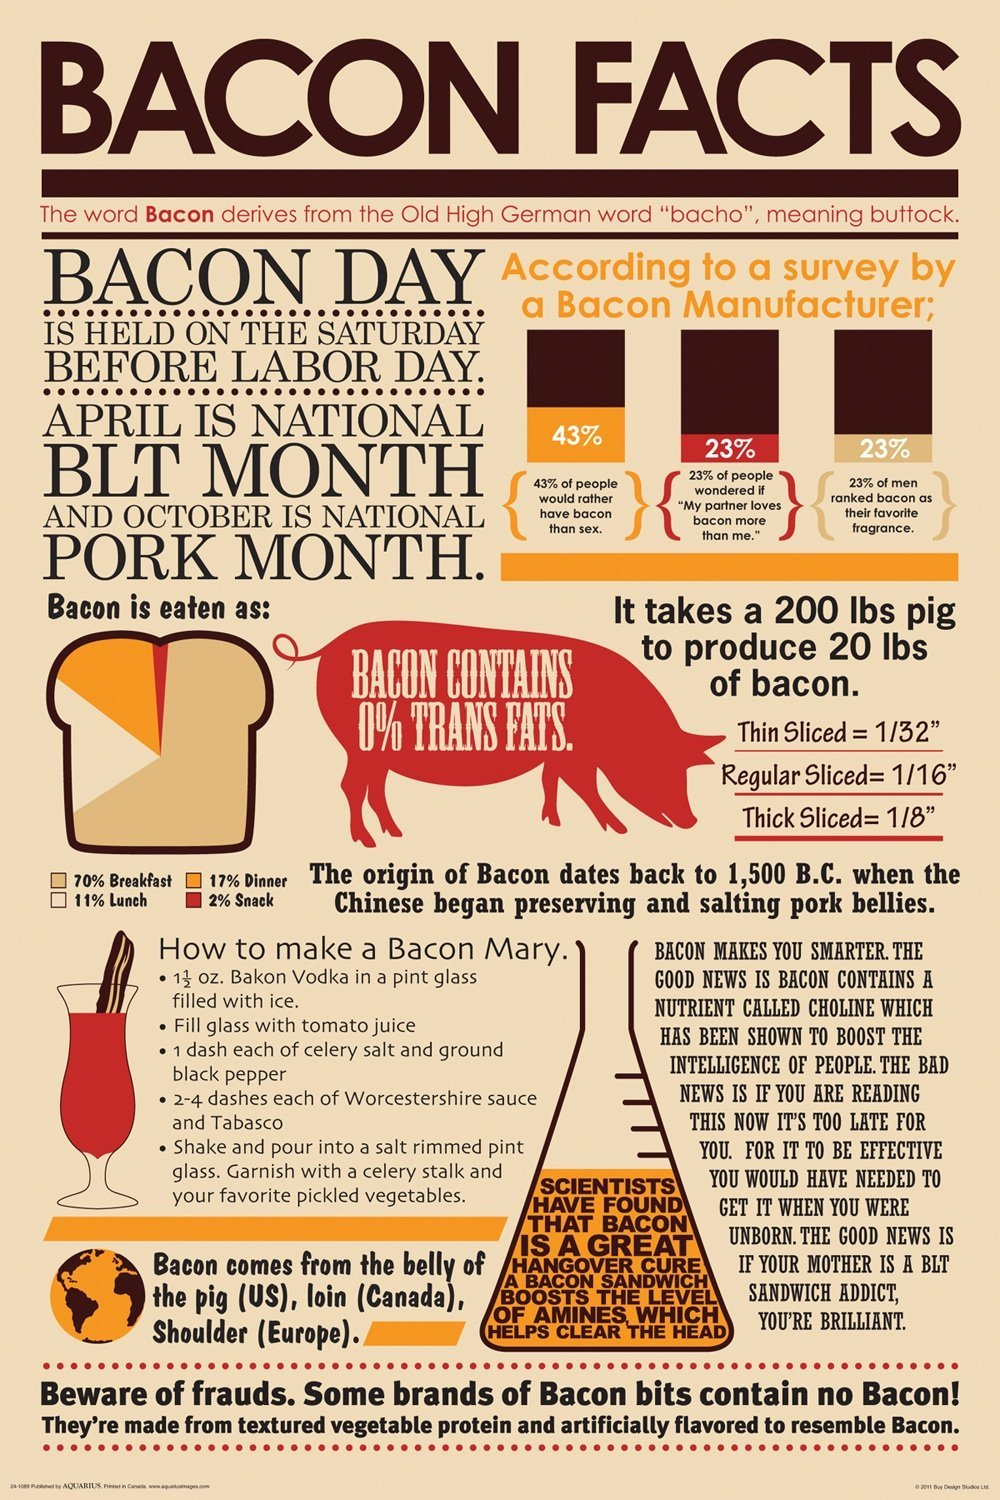
\includegraphics[width=0.5\linewidth]{img/tableDetection/readingOrderIssue.jpg}
\caption{Reading order problems. Determination of correct labels is sometimes hard even for human perception.} \label{fig:readingOrderProblems}
\end{figure}

\begin{figure}[t]
\centering
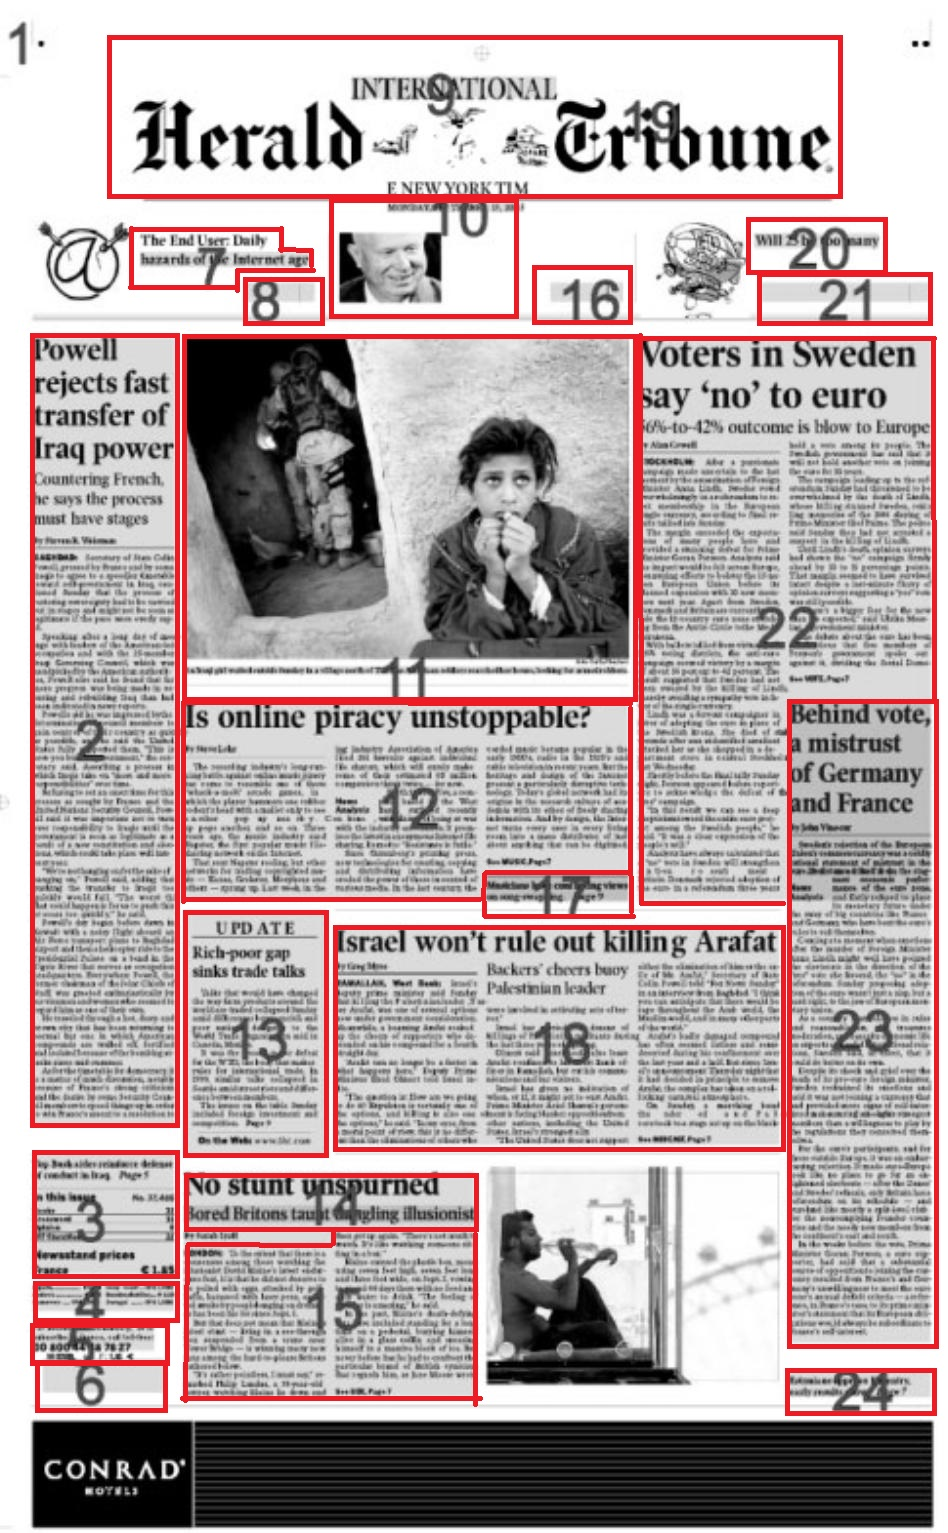
\includegraphics[width=0.5\linewidth]{img/tableDetection/readingOrder.jpg}
\caption{An example of layout analysis~\citep{hadjar2004xed}.}
\label{fig:readingOrderExample}
\end{figure}

Various heuristics are used for the determination of labels~\cite{logicalLayoutTemplate}. In the following list, we overview several of the most widely used:

\begin{itemize}
\item[\emph{Templates}]

The most simple and basic approach is the technique of the already mentioned templates. It is based on a limited number of predefined document layouts (\emph{templates}), which already contain the information about the structure of individual elements. An input document is then matched to these layouts. In the OCR engines that focus solely on processing a single type of documents (such as ticket validation, recipe or passport recognition, recognition of forms filled out by patients in hospitals), this process yields almost perfect results, even though it is a naive approach.

\item[\emph{Rule-based approaches}]

A human reader often determines the logical succession of document elements by font settings and locations of the elements. Rule-based approaches take advantage of this fact and create heuristic ``rules'' that determine the type of the element. For example, a rule for a page header could be ``has the smallest y-axis value, has font size above 22pt, is bold, and is the only element on its line''.

\item[\emph{Syntactic methods}]

These methods present the structure used for element labeling in a form of a set of formal (usually context free) grammars. These grammars contain rules for aggregating pixels into more structured entities until they form logical objects. Parsers for a syntactic analysis are automatically obtained from these grammars. They are then used to perform the actual labeling of the detected elements.

\item[\emph{Machine learning}]

Already mentioned in this thesis, a non-heuristic approach to logical layout analysis is the use of neural networks. Given enough information and time for training, the networks are able to determine the labeling on their own.

There exist various techniques of machine learning, distinguished by the way the neural networks are trained. For example, a neural network can be given a set of rules and input images, which leads the learning process to produce results similar to human observation. Also, it can be solely reliant on raw physical data and itself.

\end{itemize}

Worth mentioning are also techniques like \emph{Blackboard system}, \emph{Description language} or methods based on \emph{Hidden Markov Models}~\cite{logicalLayoutOther}.

Layout analysis is a crucial part of almost every OCR engine. If either geometric or logical layout analysis fails, the input of the recognition engine might contain corrupted data. This might lead to a significantly lower accuracy of the recognition process. 

Table recognition utilizes the output of layout analysis and extracts table related information, such as table cells, headers and footers, from it. Other elements are discarded (e.g. floating text, graphics), as they are considered worthless for the purposes of table recognition.

\section{Table recognition}

The goal of table recognition is to determine if a table even is present on a page, and if yes, where and what its content is. This process is often divided into two parts --- \emph{table detection} and \emph{table decomposition}, with table detection determining the presence and placement of a table, and table decomposition analyzing its content and producing a meaningful structure of its representation. In our thesis, we approach the table recognition problem as a whole, as usually, both parts benefit from reusing each others outputs.

Although obtaining the elements of a simple $m{\times}n$ grid is an easy task achieved by a simple line detection algorithm (e.g. Hough transform~\cite{houghTransform}), the absence of cell borders requires more complicated heuristics. Moreover, tables that contain cells of different sizes, various numbers of cells in different rows, complicated headers or footers, multi-line cells and many more also require more complex solutions. We present a few of these possible obstacles in~\cref{fig:tableRecognitionObstacles}.

\begin{figure}[t]
\centering
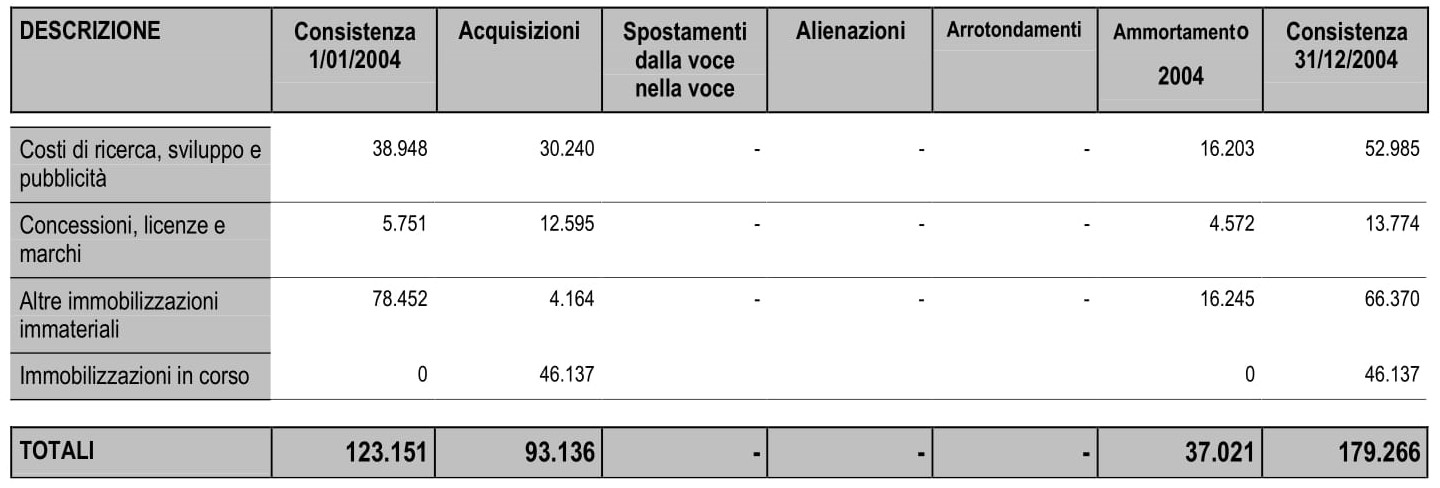
\includegraphics[width=0.7\linewidth]{img/tableDetection/recognitionProblematic.jpg}
\caption{Several common problems occurring during table recognition: missing horizontal and vertical lines; missing information in cells; multi-line cells in the first column and header row; different alignment of header and content cells.}
\label{fig:tableRecognitionObstacles}
\end{figure}

In this section, we overview some of the existing table recognition algorithms. For the purposes of this thesis, we specifically focus on the table recognition implementation of the Tesseract engine.

\subsection{Tesseract table recognition} \label{tableFind}

The Tesseract engine has been originally used for character detection. Over the years, many features have been added, including a \textsc{TableFind} algorithm for table detection and recognition.

\citet{tableDetHeterogeneous} based the TableFind recognition algorithm on already existing Tesseract's features, including layout analysis (described in~\cref{sectionTessPageSegm}) and character detection (\cref{tesseractCharacterRecognition}). Following are the individual steps of the algorithm, along with their visualization in~\cref{fig:tesseractTableRecognition}: 

\begin{enumerate}
\item \emph{Layout analysis}

First, layout analysis is performed by \emph{tab-stop detection}~(\cref{sectionTessPageSegm}) included in the Tesseract library. The results of this step include not only a list of segmented blocks, but also the column layout (~\cref{fig:tessTableDet1}) and column partitions (sequences of connected components of the same type --- like text, image --- that do not cross any tab-line, presented in~\cref{fig:tessTableDet2}).

\item \emph{Identification of table partitions}

With the page layout available, TableFind tries to identify text column partitions that could possibly belong to a table --- \emph{table partitions}. This process is based on heuristics, by identifying column partitions that contain at least one large gap between their connected components, consist of only one word, or overlap with other partitions along the y-axis.

This stage of the algorithm is performed quite aggressively, so although this process returns the desired table partitions, it also produces a lot of false positives, such as considering section headings, page headers, footers, equations, etc., as tables. Most of these unwanted partitions are then removed by a heuristic filter. However, as presented in~\cref{fig:tessTableDet3}, the presence of minor mistakes is not completely eliminated.

\item \emph{Detection of table columns}

As shown in~\cref{fig:tessTableDet4}, vertically aligned partitions are grouped into a single column. Columns with only one partition are then removed. 

\item \emph{Table construction}

The goal of table construction is to group table columns into a table. Here, TableFind assumes that flowing text does not share space with a table along the y-axis. Therefore, boundaries of table columns are expanded along the y-axis to the borders of the page columns that contain them. In result, bounding boxes are created for whole tables. Tables that span across multiple page columns are detected only if a table column exists that belongs to all of these page columns.

\item \emph{Removal of false positives}

Because of relatively greedy heuristic used in the previous step, non-tabular content may be falsely identified in a table. Therefore, TableFind finally removes tables with only one column. This produces the final result (\cref{fig:tessTableDet5}).

\end{enumerate}

The algorithm has been proved to have a 86\% precision. The biggest problems have shown to be full-page tables, often resulting in over or under-segmentation, partial detection or detection of false positives~\citep{tableDetHeterogeneous}.

Another problem with TableFind is that currently, there exists no simple command that a user could run to see the output of this algorithm. To actually detect a table, a user must first write its own program that uses the functions of the added Tesseract table recognition files. Then, he needs to process the data the library returns and output them in a meaningful format, which requires a non-trivial knowledge of the Tesseract implementation.

We further present the results of this algorithm in~\cref{resultsTableFind}, where we compare them to our implementation.
   
\begin{figure}
\centering
\begin{subfigure}{0.30\textwidth}
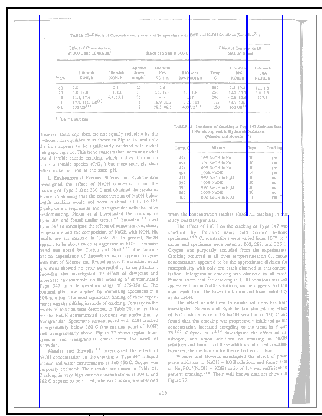
\includegraphics[width=\linewidth]{img/tableDetection/tableDetectionColumns.pdf}
\caption{Column layout.}
\label{fig:tessTableDet1}
\end{subfigure}
\quad
\begin{subfigure}{0.30\textwidth}
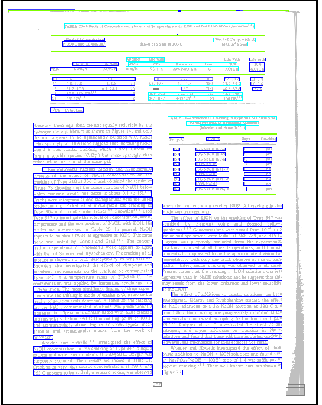
\includegraphics[width=\linewidth]{img/tableDetection/tableDetectionPartitions.pdf}
\caption{Column partitions.}
\label{fig:tessTableDet2}
\end{subfigure}
\quad
\begin{subfigure}{0.30\textwidth}
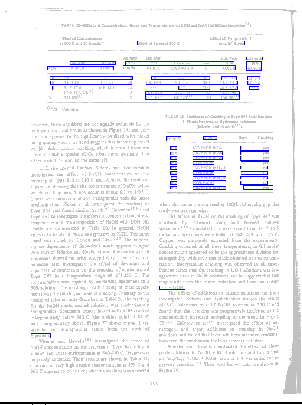
\includegraphics[width=\linewidth]{img/tableDetection/tableDetectionCandidate.pdf}
\caption{Candidate table partitions.}
\label{fig:tessTableDet3}
\end{subfigure}
\\
\begin{subfigure}{0.30\textwidth}
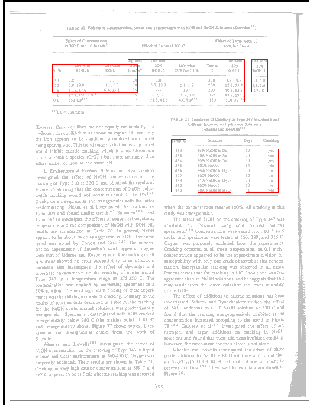
\includegraphics[width=\linewidth]{img/tableDetection/tableDetectionTabCols.pdf}
\caption{Table columns.}
\label{fig:tessTableDet4}
\end{subfigure}
\quad
\begin{subfigure}{0.30\textwidth}
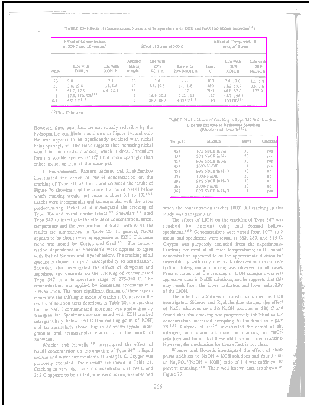
\includegraphics[width=\linewidth]{img/tableDetection/tableDetectionResult.pdf}
\caption{Detected table regions.}
\label{fig:tessTableDet5}
\end{subfigure}
\caption{The process of Tesseract table recognition~\cite{tableDetHeterogeneous}.}
\label{fig:tesseractTableRecognition}
\end{figure}

\subsection{Other existing approaches}

In addition to the TableFind algorithm, there exist various heuristic approaches for table detection. In this section, we overview several of them, including their advantages and disadvantages. Specifically, we focus on T-Recs table recognition system~\citep{TRecs}, Medium-independent table detection~\citep{MediumTable}, pdf2table project~\cite{pdf2table} and an approach based on a hierarchical MXY tree page representation~\citep{tableDetectCesarini}. However, multiple other approaches also exist. Worth mentioning is also, for example, sparse line detection~\cite{sparseLineDetection}, which already uses principles of machine learning. Some of the other methods are briefly reviewed by~\citet{otherDetection1} or~\citet{otherDetection2}.

One of the first approaches to table recognition was presented by the \emph{T-recs} table recognition system~\cite{TRecs}, which is based on a bottom-up approach of clustering word bounding boxes and building a ``segmentation graph''. This segments the page into different regions, which are then evaluated by certain heuristic criteria for tables. Although widely popular in the 90s, this technique has several setbacks. T-Recs is controlled by a set of numerical parameters, which need to be adjusted manually by the user according to the layout of the page. Moreover, it yields unsatisfactory results on multi-column documents.

Another algorithm was described by~\citet{MediumTable}. In single-column documents, a page can be easily segmented into individual textlines. The table detection problem is then perceived as an optimization problem, where the start and end textlines that belong to a table are identified by optimizing some quality function. However, this approach fails on multi-column documents, and on documents that contain more than one table.

\citet{tableDetectCesarini} describe an approach based on hierarchical MXY-tree-like representation. The presence of a table is determined by searching the tree for parallel lines that contain white spaces, and other perpendicular lines between them, which indicate cell borders. Located tables are merged on the basis of proximity and similarity criteria. However, this approach fails if no lines in tables are present.

Method presented by the \emph{pdf2table} project~\cite{pdf2table} is based on assigning each text object of the page its positional attributes. By the evaluation of these attributes, text objects are then merged into single-lines (lines with only one text object), multi-lines (lines with more than one text object) and multi-line blocks (multiple multi-lines merged together). The table detection algorithm then merges the multi-line blocks that may belong to the same table, with the help of a heuristic threshold that determines the greatest number of single-line objects between two multi-line blocks possible. This method also assumes the input to be a single-column document. Despite of that, the user can manually adjust the information about the number of columns, which yields more accurate results.